\documentclass[oneside]{VUMIFPSkursinis}
\usepackage{algorithmicx}
\usepackage{algorithm}
\usepackage{algpseudocode}
\usepackage{amsfonts}
\usepackage{float}
\usepackage{amsmath}
\usepackage{bm}
\usepackage{caption}
\usepackage{color}
\usepackage{float}
\usepackage{graphicx}
\usepackage{listings}
\usepackage{subfig}
\usepackage{ltablex}
\usepackage{longtable}
\usepackage{wrapfig}
\usepackage{subfig}
\usepackage{pbox}
\renewcommand{\labelenumii}{\theenumii}
\renewcommand{\theenumii}{\theenumi.\arabic{enumii}.}
\renewcommand{\labelenumiii}{\theenumiii}
\renewcommand{\theenumiii}{\theenumii\arabic{enumiii}.}
\newcolumntype{P}[1]{>{\centering\arraybackslash}p{#1}}
\usepackage[%  
    colorlinks=true,
    linkcolor=black
]{hyperref}
\university{Vilniaus universitetas}
\faculty{Matematikos ir informatikos fakultetas}
\department{Programų sistemų katedra}
\papertype{Programų sistemų inžinerija II laboratorinis darbas II}
\title{Reikalavimų apibrėžimas}
\titleineng{Requirements specification}
\status{2 kurso 3 grupės studentai}



\supervisor{Audronė Lupeikienė, M. Darbuot., Dr.}
\date{Vilnius – \the\year}

\bibliography{bibliografija}

\begin{document}
\maketitle
\tableofcontents

\section{Anotacija}
	\begin{itemize}
		\item Matas Savickis
		\item Greta Pyrantaitė
		\item Justas Tvarijonas
		\item Rytautas Kvašinskas
		\item Tomas Kiziela
	\end{itemize}

\section {Reikalavimai}

\subsubsection{Pataisyta funkcinių reikalavimų specifikacija}
\begin{enumerate}
	\item Sistema seka vartotojų laiką, praleistą trasoje, pasinaudodama sekimo prietaisu.
	\item Sistema suteikia galimybę vartotojui įsidėti pinigų į virtualią piniginę.
	\begin{enumerate}
		\item Top-up metodu.
		\item Pervedimo būdu.
	\end{enumerate}
	\item Sekimo prietaisas fiksuoja greičiausią laiką, per kurį vartotojas įveikė trasą.
	\begin{enumerate}
		\item sistema saugo greičiausią laiką, per kurį vartotojas įveikė trasą.
	\end{enumerate}
	\item Vartotojo trasų laikai rodomi internetinėje aplikacijoje.
	\item Sistema suteikia vartotojui galimybę tvarkyti savo paskyrą.
	\begin{enumerate}
		\item Prisijungti.
		\item Atsijungti.
		\item Keisti asmeninius duomenis.
		\item Keisti paskyros slaptažodį.
	\end{enumerate}
	\item Sistema internetinės aplikacijos pagalba vartotojui suteikia galimybę peržiūrėti orus.
	\begin{enumerate}
		\item Sistema turi pateikti dabartines oro sąlygas.
		\item Sistema turi pateikti ateinančių dienų orų prognozę.
		\begin{enumerate}
			\item temperaturą.
			\item drėgmę.
			\item kritulius.
			\item vėjo greitį.
		\end{enumerate}
	\end{enumerate}
	\item Internetinėje aplikacijoje vartotojas gali rašyti žinutes kitiems kurorto svečiams, administracijai ir maisto į kambarį tarnybai.
	\item Sistema vartotojui suteikia galimybę rašyti atsiliepimą apie jo viešnagę kurorte ir skirti viešą vertinimą kurortui.
	\item Internetinė aplikacija administratoriui suteikia galimybę tvarkyti duomenis.
	\begin{enumerate}
		\item Tvarkyti trasų duomenis.
		\item Tvarkyti kurorto statistinius duomenis.
		\item Tvarkyti atsiliepimus.
	\end{enumerate}
	\item Internetinė aplikacija suteikia vartotojui galimybę peržvlegti statistiką.
	\begin{enumerate}
		\item Vartotojas turi galėti peržiūrėti savo statistiką.
		\item Vartotojas turi galėti peržiūrėti kurorto statistiką, jeigu ji patvirtinta administratoriaus.
		\begin{enumerate}
			\item Administratorius turi galėti patvirtinti arba atmesti naują statistiką apie kurortą.
		\end{enumerate}
	\end{enumerate}
	\item Sistemoja per internetinę aplikaciją vartotojui suteikia galimybę peržiūrėti paslaugų kainas, tiekėjų sąrašą ir kiekvienos įrangos technines charakteristikas.
	\item Sistema administratoriui suteikia galimybę skaityti sutarčių ataskaitas.
	\item Sistema per aplikaciją vartotojui suteikia galimybę užsisakyti paslaugas.
	\begin{enumerate}
		\item Užsisakyti maisto į viešbučio kambarį.
		\item Rezervuoti slidinėjimo įrangą.
	\end{enumerate}
	\item Sistema internetinės aplikacijos pagalba leidžia vartotojui peržiūrėti visas jo pasirašytas sutartis.
	\item Vartotojas turi galimybę per internetinę aplikaciją užrezervuoti slidinėjimo trasą nurodant: trasos pavadinimą, telefono numerį, slidinėtojų skaičių ir rezervacijos laikotarpį.
	\item Vartotojas gali matyti informaciją apie slidinėjimo trasą: pavadinimą, sunkumą, rūšį, nuomos kainą, užimtumą.
	\item \textit{Sistema vartotojui suteikia galimybę peržiūrėti jo užsakytas paslaugas}
	\item \textit{Sistema administratoriui suteikia galimybę pamatyti trasas rezervavusių žmonių sąrašą}
	\item Sistema suteikia galimybę keisti vertinimą.
	\item Sistema suteikia galimybę pasirinkti laikotarpį, kuriuo filtruoti lankytas trasas.

\end{enumerate}

\subsubsection{Pataisyta nefunkcinių reikalavimų specifikacija}
\begin{enumerate}

	
	\item Sistema neleidžia vertinti kurorto kelis kartus tam pačiam asmeniui dažniau, nei kartą per 2 mėnesius.

	\item Atsiskaitinėjant vartotojas gali identifikuotis piršto antspaudu.
	\item Sistema leidžia vartotojui už paslaugas atsiskaityti e-bankininkyste.
	\item Slidinėjimo trasų įrangos bei kambarių pavadinimams maksimaliai skiriama 64 simboliai
	\item Slidinėjimo trasos ilgis vaiduojamas vieno skaičiaus po kablelio tikslumu
	\begin{enumerate}
		\item Ilgio matavimo vienetas - kilometras
	\end{enumerate}
	\item Slidinėjimo trasos statumas vaizduojamas vieno skaičio po kablelio tikslumu
	\begin{enumerate}
		\item Statumo matavimo vienetas - procentai
	\end{enumerate}
	\item Slidinėjimo trasų, įrangos bei apgyvendinimo įstaigos laisvų vietų skaičius rodomas vienetų tikslumu.
	\item Slidinėjimo trasų, įrangos bei apgyvendinimo įstaigos kainos pateikiamos centų po kablelio tikslumu (10,11eu)
	\item Data turi būti vaizduojama formatu YYYY-MM-DD
	\begin{enumerate}
		\item YYYY - metai
		\item MM - mėnuo
		\item DD - diena
	\end{enumerate}
	\item Laikas turi būti vaizduojamas formatu hh:mm 24 valandų formatu (21:47)
	\begin{enumerate}
		\item hh - valandos 24 valandų formatu
		\item mm - minutės
	\end{enumerate}
	\item Vartotojo vardui, pavardei, elektroniniam paštui, slaptažodžiui registracijos formoje maksimaliai skiriama 64 simboliai. Taip pat registracijos formoje vartotojams reikia įvesti slaptažodį, kuriam maksimaliai skiriama 512 simboliai.
	\item Vartotojo raktas sugeneruojamas pagal GUID
	\item Vartotojo elektroniniam paštui prisijungiant skiriama 64 simboliai o slaptažodžiui 512
	\item Vartotojo slaptažodis negali būti trumpesnis negu 10 simbolių
	\item Vardui, pavardei ir elektroniniam paštui rezervacijos formoje skiriama 64 simboliai
	\item Telefono numeriui rezervacijos formoje skiriama 15 simbolių
	\item Svečių skaičiui rezervacijos formoje maksimaliai skiriama 3 skaičiai
	\item Orų temperatūra rodoma vienetų tikslumu. Matavimo vienetas - celsijus
	\item Rezervacijos/užsakymo/sutarties numeris pateikiamas vienetų tikslumu
	\item Įrangos dydžiai - europietiški. Vaizduojama vienetų tikslumu
	\item Keičiant naršyklės dydį, tinklapio vaizdas pritaikomas automatiškai(Responsive design).
	\item Sistema turi veikti 95proc laiko per dieną. Tai yra leidžiama neveikti 1 valandą 10 min.	
	\item Registruojant naują vartotoją sistema turi patikrinti, ar teisingai įvesti jo duomenys.
	\item Prisijungiant vartotojui sistema turi patikrinti, ar įvesti duomenys teisingi.
	\item Vartotojui rezervuojant paslaugas sistema turi patikrinti, ar duomenys įvesti korektiškai
	\item Vartotojui rezervuojant paslaugas sistema rezervacijai turi priskirti unikalų numerį.
	\item Modifikuojama tinklapio atsarginė kopija po kiekvieno informacijos atnaujinimo apie slidinėjimo kurortą, orų prognozes, slidinėjimo trasas, įrangą, apgyvendinimo įstaigą, jų užimtumą bei po kiekvienos esybės registracijos ir įvestos informacijos pakeitimo.
	\item Bandant pildyti laukus ne pagal pateiktus reikalavimus, užklausa negali būti įvykdyta.
	\item Sistemoje turi būti įdiegtos apsaugos priemonės nuo duomenų sugadinimo, praradimo, klaidingų duomenų įvedimo į duomenų bazėje.
	\item Po kiekvienos sėkmingos operacijos pakeitimai turi būti išsaugoti duomenų bazėje.
	\item Nepavykus prisijungti arba negavus duomenų iš duomenų bazės, sistema turi informuoti vartotoją, parodydamas klaidos pranešimą
	\item Didžiausia leistina tinklalapio apkrova yra 10000 vartotojų vienu metu
	\item Tinklalapio didžiausias leistinas reakcijos laikas, neįvertinant interneto greičio, turi būti ne didesnis kaip 2 sekundės.
	\item Užklausos vykdymo laikas turi būti ne didesnis nei 3 sekundės
	\item Konkrečios slidinėjimo trasos, įrangos, kambario, jų užimtumo paieškai duomenų bazėje turi būti sugaišta ne ilgiau nei 3 sekundės
	\item Tinklapis pasiekiamas prisijungiant iš bet kurio IP adreso
	\item Pradinėje sistemoje turi būti administratoriaus prisijungimo duomenys
	\item Pasirinkimų lentelė turi turėti bent 5 pradines užpildytas eilutes su informacija apie slidinėjimo trasas, įrangą, kambarius. Šią informaciją įveda įgaliotas įmonės administratorius interfeisu.
	\item Sistemos turi funkcionuoti lietuvių ir anglų kalbomis
	\item Įmonės darbuotojai turi būti apmokomi naudotis sistema
	\item Tinkalpyje negali būti klaidinančios informacijos
	\item Pakeitimai turi būti įvykdyti ne vėliau nei per 7 darbo dienas po sėkmingo testavimo.
	\item Visi vartotojo atliekami veiksmai turi būti saugomi laikinoje duomenų bazėje, kad atradus klaidą tinklalapyje būtų galima testavimo metu atkurti konkrečia klaidą
	\item Pastebėtos ar esybės praneštos klaidos turi būti ištaisytos kaip galima greičiau.
	\item Į vartotojo atsiųstus laiškus su pastebėjimai ir skundais reikia atsakyti automatine žinute.
	\item Sistema atnaujinti reikia tuo metu, kai yra mažiausias vartotojų srautas
	\item Internetinė aplikacija turi veikti bet kuriame įrenginyje, kuris turi naršyklę, palaikančią HTML5 standartą.
	\item Vartotojui prisijungiant prie sistemos vykdoma jo indentifikacija.
	\item Duomenų bazėje saugomas slaptažodžių maišos kodas, sumaišytas SHA512 algoritmu.
	\item Visi duomenys apie sistemą saugomi duomenų bazėje, o prie jos prieigą turi tik įgalioti asmenys.
	\item Atsarginė duomenų bazės kopija turi būti daroma reguliariai kas 7 darbo dienas.
	\item Jeigu esybė neaktyvi ilgiau nei 15 minučių, vartotojas automatiškai atjungiamas.
	\item Kuriant sistemą projekto komandai draudžiama naudotis nelegalia programine įranga
	\item Duomenų perdavimas ir saugojimas neturi pažeisti LR asmens duomenų teisinės apsaugos įstatymo.
	\item Esybių asmeniniai duomenys turi būti įslaptinti t.y. tinklapyje negali būti saugomi nekoduoti duomenys
	\item Minimali sąskaitos papildymo suma 3€

\end{enumerate}


\pagebreak

\subsection{Pataisytas dalykinės srities diagrama}
\begin{figure}[h]
    \centering
    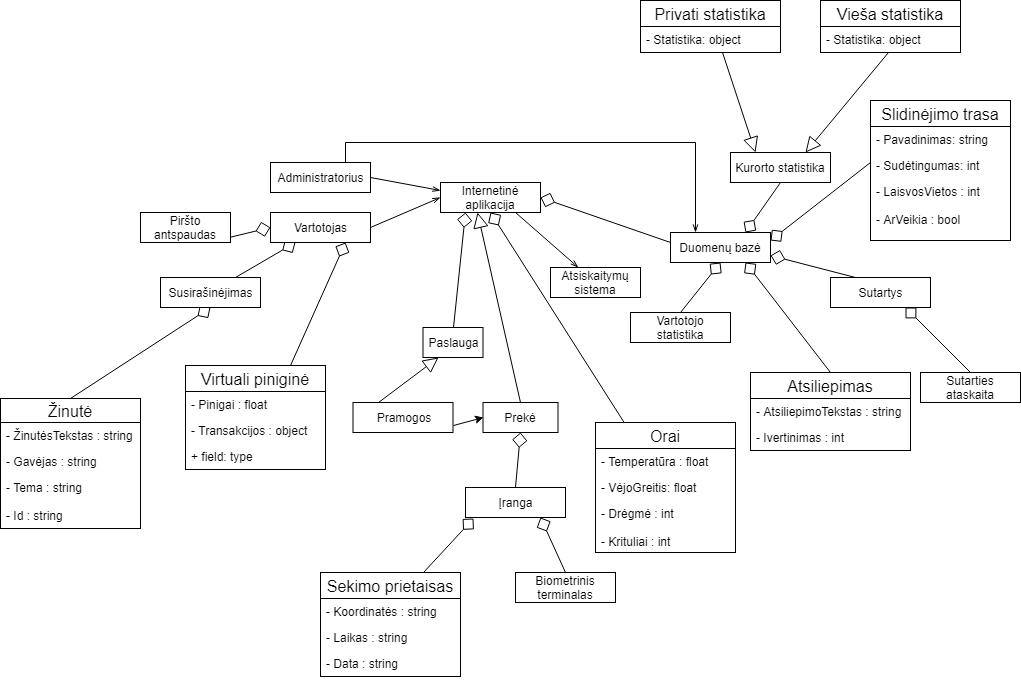
\includegraphics[width=0.80\textwidth]{DomainModelFixed.png}
    \caption{Pataisyta dalykines srities diagrama}
    \label{fig:Pataisyta dalykinės srities diagrama}
\end{figure}
\subsection{Use case peržiūra}


\subsection{Pakeitimai}

\begin{longtable}{ | p{0.2\textwidth}|p{0.2\textwidth}|p{0.5\textwidth}| }  \hline
	Pataisymo nr. & Use case numeris & Klaidos aprašas \\ \hline
	1 & 1 & Ištrintas užduotyje esantis NFR ir pridėtas į NFR sąrašą\\ \hline
	2 & 2 & Ištrintas užduotyje esantis NFR, pakeistas į FR ir pridėtas į FR sąrašą\\ \hline
	3 & 5 & Aktorius pakeistas iš administratoriaus į vartotoją\\ \hline
	4 & 6 & Pakeisti alternatyvūs scenarijai, pataisytas pagrindinis scenarijus\\ \hline
	5 & 8 & Pridėtas alternatyvus scenarijus\\ \hline
	6 & 14 & Išimtas vienas metodas, kadangi turi būti rodoma tik dabartinės trasos informacija\\ \hline
\end{longtable}


\section{Dalykinė sritis}
\subsection{Dalykinės srities žodynas}

\begin{enumerate}
	\item Internetinė aplikacija - Mūsų kuriama android programėlė
	\item Administratorius - Sistemą prižiūrintis žmogus
	\item Vartotojas - Slidinėjimo kurorto klientas, naudojantis programėlę
	\item Susirašinėjimas - Dviejų vartotojų žinučių grandinė
	\item Žinutė - Simbolių rinkinys, kurį vienas vartotojas siunčia kitam
	\item Virtuali piniginė - Piniginė, kurioje esančiais pinigais galima atsiskaityti už pramogas
	\item Kaina - Pinigų suma už prekę ar paslaugą
	\item Sekimo prietaisas - Įrenginys, siunčiantis savo poziciją sistemai
	\item Biometrinis terminalas - Įrenginys, kuris skenuoja piršto antspaudą
	\item Tiekėjai - Žmonės, kurie tiekia įrangą
	\item Orai - Informacija apie orų prognozę
	\item Atsiskaitymų sistema - Sistema, kuri apdoroja bankinius pinigų pervedimus
	\item Duomenų bazė - Organizuota duomenų struktūra
	\item Vartotojo statistika - Duomenys, renkami apie vartotoją
	\item Atsiliepimas - Simbolių rinkinys, parašytas vartotojo apie aplikaciją
	\item Sutartys - Rašytinis susitarimas tarp vartotojo ir slidinėjimo kurorto
	\item Slidinėjimo trasos - Informacija apie slidinėjimo trasas
	\item Kurorto statistika - Duomenys renkami apie kurortą
\end{enumerate}
\pagebreak

\subsection{dalykinies srities modelio diagrama}
\begin{figure}[h]
    \centering
    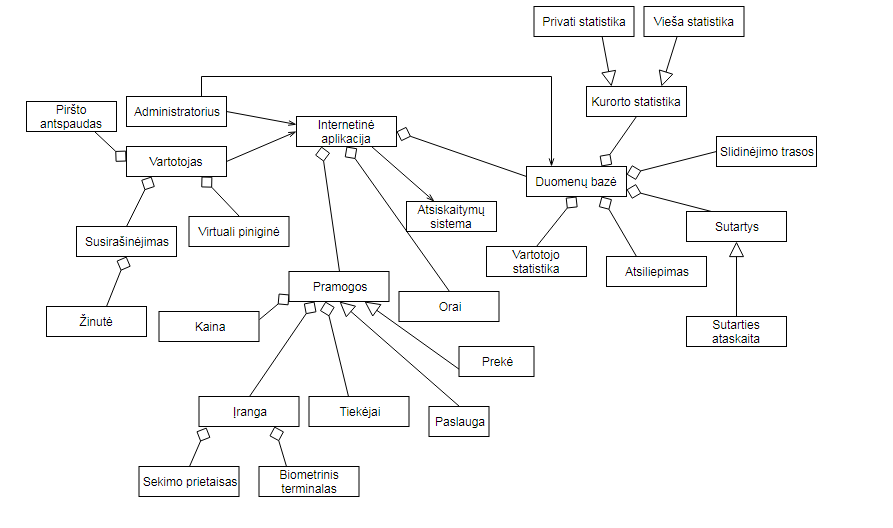
\includegraphics[width=1\textwidth]{DomainModel.png}
    \caption{Domain model diagrama}
    \label{fig:DomainModel}
\end{figure}
\pagebreak

\subsection{Reikalavimų/esybių atsekamumo matrica}	
\begin{figure}[h]
    \centering
    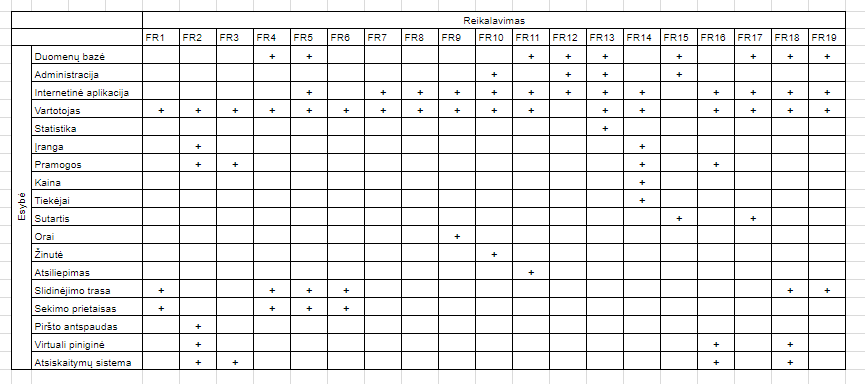
\includegraphics[width=1\textwidth]{Reikalavimai_Esybes.png}
    \caption{Reikalavimų/Esybių atsekamumo matrica}
    \label{fig:r/e_matrica}
\end{figure}




\section{Užduotys}
\subsection{Use case diagramos}
\begin{figure}[h]
    \centering
    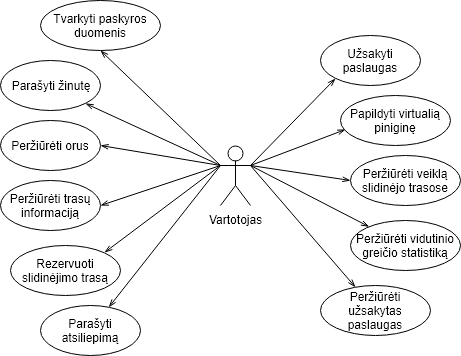
\includegraphics[width=0.75\textwidth]{useCaseVartotojas.png}
    \caption{Vartotojo užduočių diagrama}
    \label{fig:VartotojoUseCasel}
\end{figure}
\vskip 1cm
\begin{figure}[h]
    \centering
    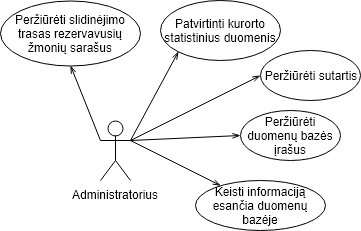
\includegraphics[width=0.65\textwidth]{useCaseAdministratorius.png}
    \caption{Administratoriaus užduočių diagrama}
    \label{fig:AdministratoriausUseCase}
\end{figure}

\break

\section{Robastiškumo analizė}
\begin{figure}[h]
    \centering
    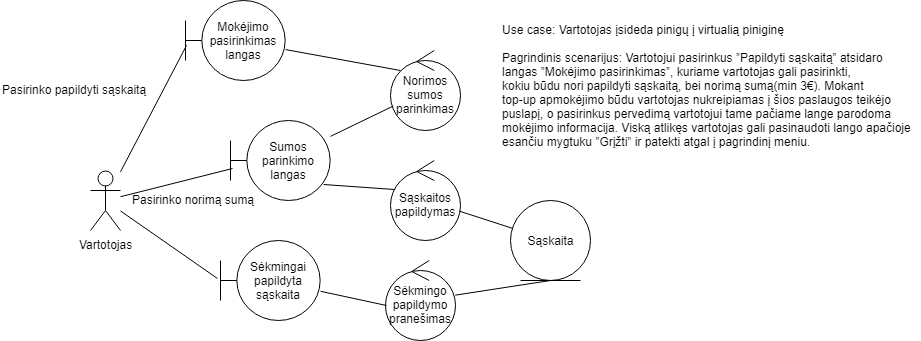
\includegraphics[width=1.0\textwidth]{Rob1.png}
    \caption{UC: Vartotojas įsideda pinigų į virtualią piniginę}
    \label{fig:rob1}
\end{figure}
\vskip 1cm

\begin{figure}[h]
    \centering
    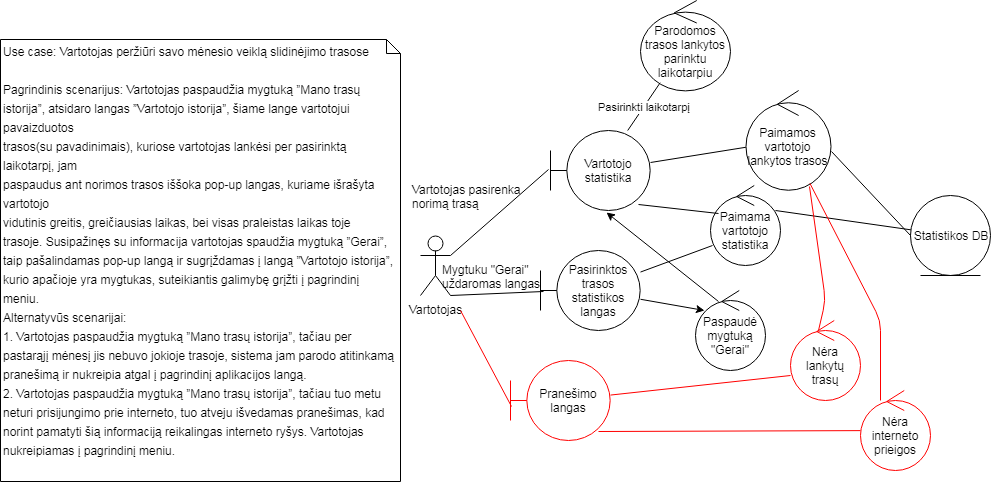
\includegraphics[width=1.0\textwidth]{rob2.png}
    \caption{UC: Vartotojas peržiūri savo mėnesio veiklą slidinėjimo trasose}
    \label{fig:rob2}
\end{figure}

\begin{figure}[h]
    \centering
    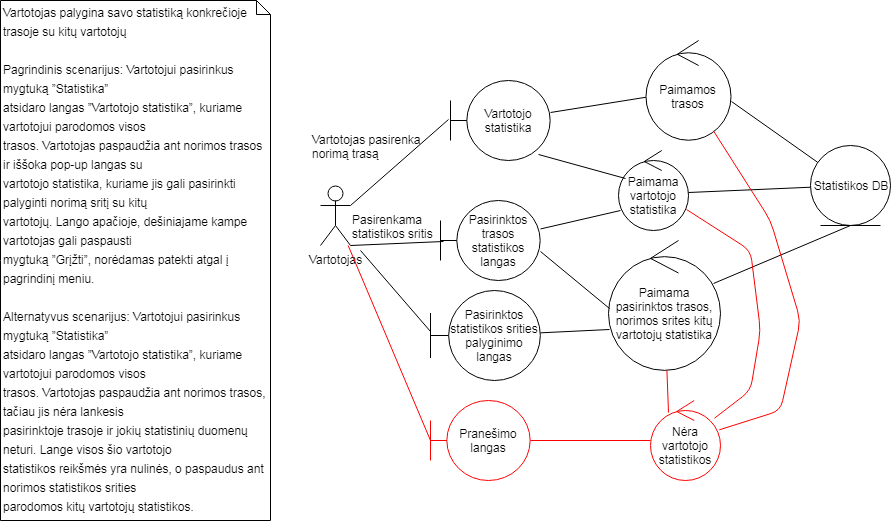
\includegraphics[width=1.0\textwidth]{rob3.png}
    \caption{UC: Vartotojas palygina savo statistiką konkrečioje trasoje su kitų vartotojų}
    \label{fig:rob3}
\end{figure}
\vskip 1cm

\begin{figure}[h]
    \centering
    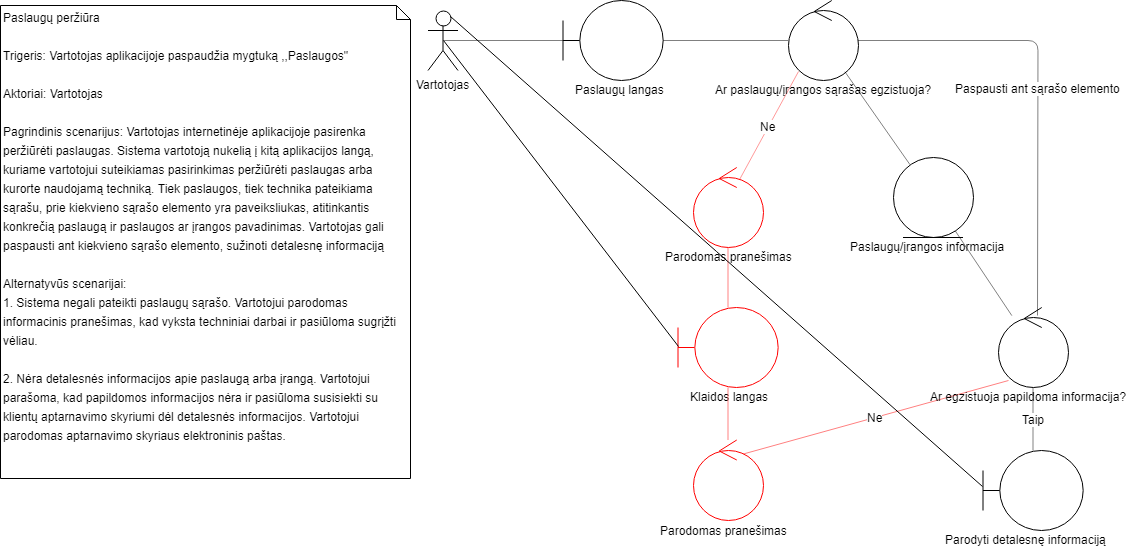
\includegraphics[width=1.0\textwidth]{Rob4.png}
    \caption{UC: Paslaugų peržiūra}
    \label{fig:rob4}
\end{figure}
\vskip 1cm

\begin{figure}[h]
    \centering
    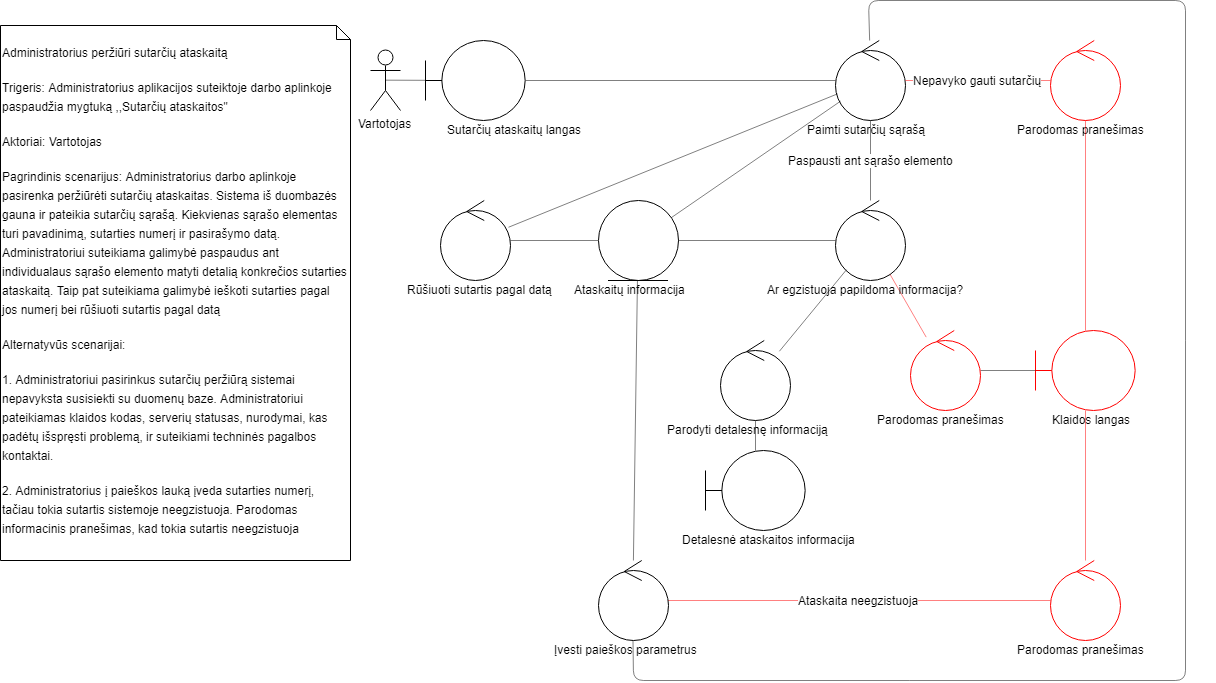
\includegraphics[width=1.0\textwidth]{Rob5.png}
    \caption{UC: Administratorius peržiūri sutarčių ataskaita}
    \label{fig:rob5}
\end{figure}
\vskip 1cm

\begin{figure}[h]
    \centering
    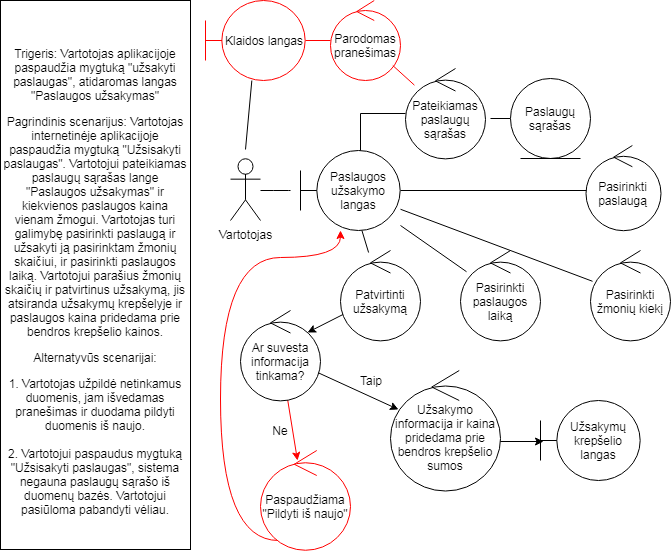
\includegraphics[width=1.0\textwidth]{rob6.png}
    \caption{UC: Paslaugų užsakymas}
    \label{fig:rob6}
\end{figure}
\vskip 1cm

\begin{figure}[h]
    \centering
    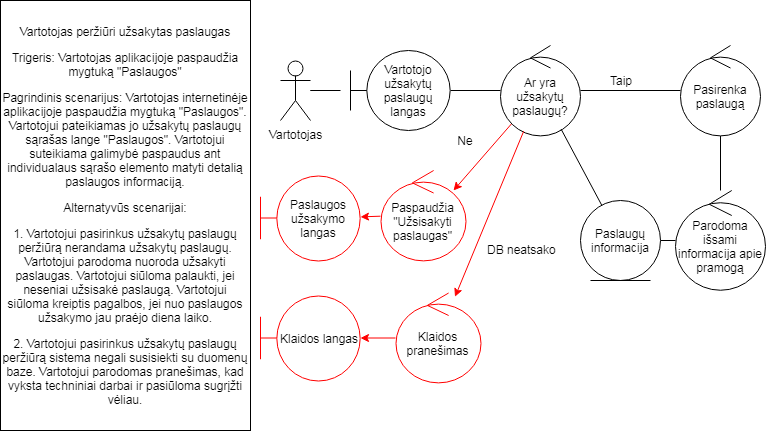
\includegraphics[width=1.0\textwidth]{rob7.png}
    \caption{UC: Vartotojas peržiūri užsakytas paslaugas}
    \label{fig:rob7}
\end{figure}
\vskip 1cm

\begin{figure}[h]
    \centering
    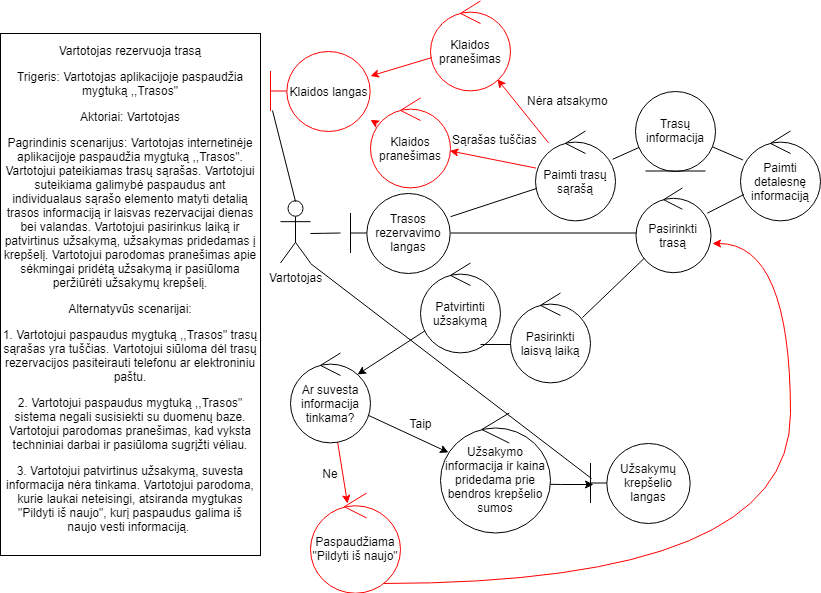
\includegraphics[width=1.0\textwidth]{rob8.png}
    \caption{UC: Vartotojas rezervuoja trasą}
    \label{fig:rob8}
\end{figure}
\vskip 1cm

\begin{figure}[h]
    \centering
    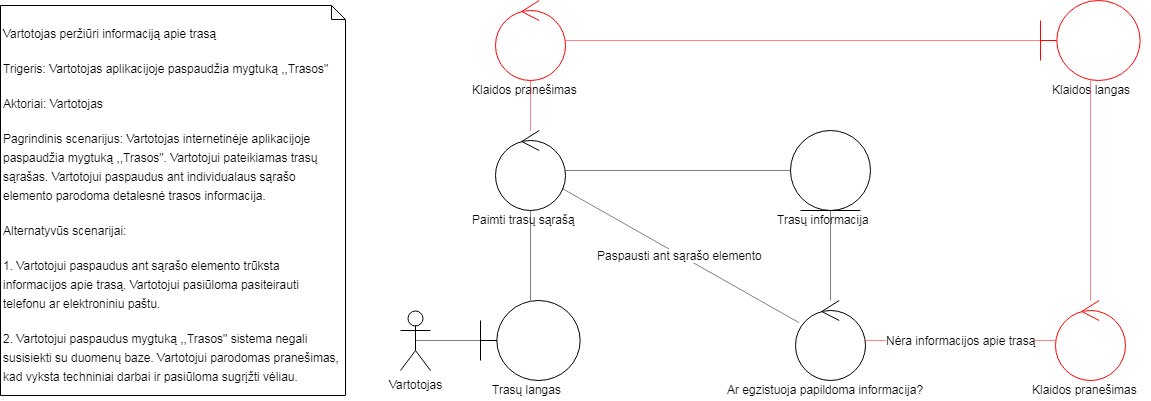
\includegraphics[width=1.0\textwidth]{Rob9.png}
    \caption{UC: Vartotojas peržiūri informaciją apie trasą}
    \label{fig:rob9}
\end{figure}
\vskip 1cm

\begin{figure}[h]
    \centering
    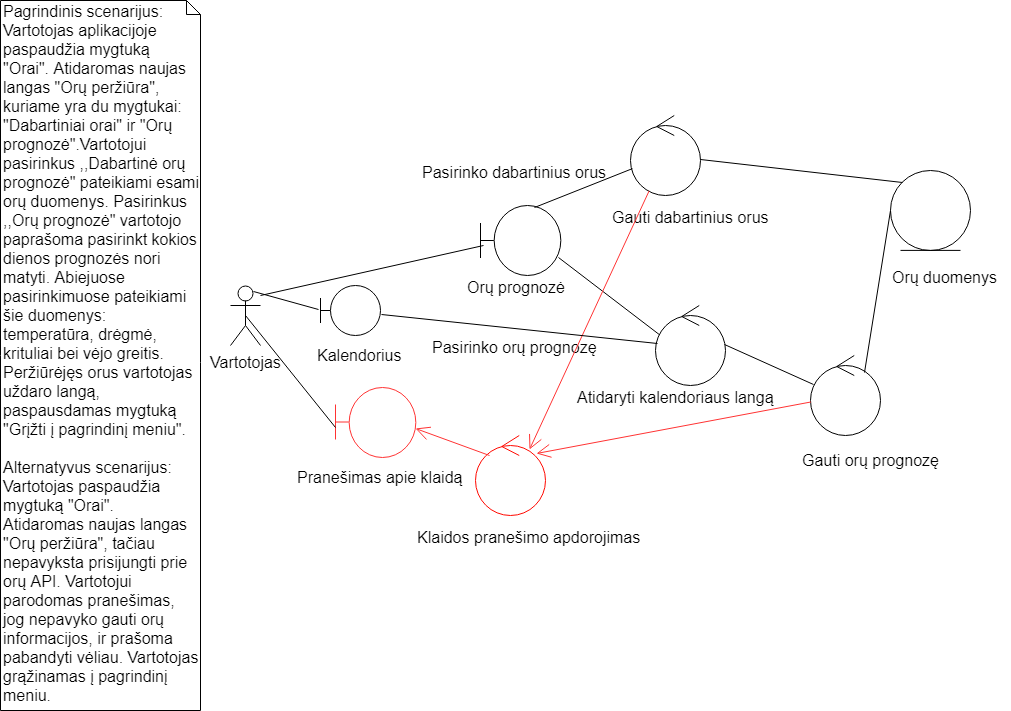
\includegraphics[width=1.0\textwidth]{Rob10.png}
    \caption{UC: Orų peržiūra}
    \label{fig:rob10}
\end{figure}
\vskip 1cm

\begin{figure}[h]
    \centering
    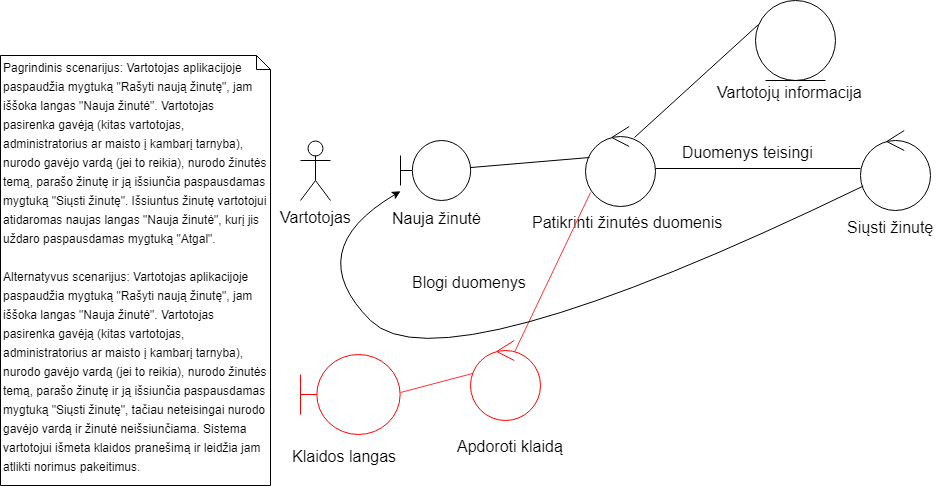
\includegraphics[width=1.0\textwidth]{Rob11.png}
    \caption{UC: Vartotojas rašo žinutę}
    \label{fig:rob11}
\end{figure}
\vskip 1cm

\begin{figure}[h]
    \centering
    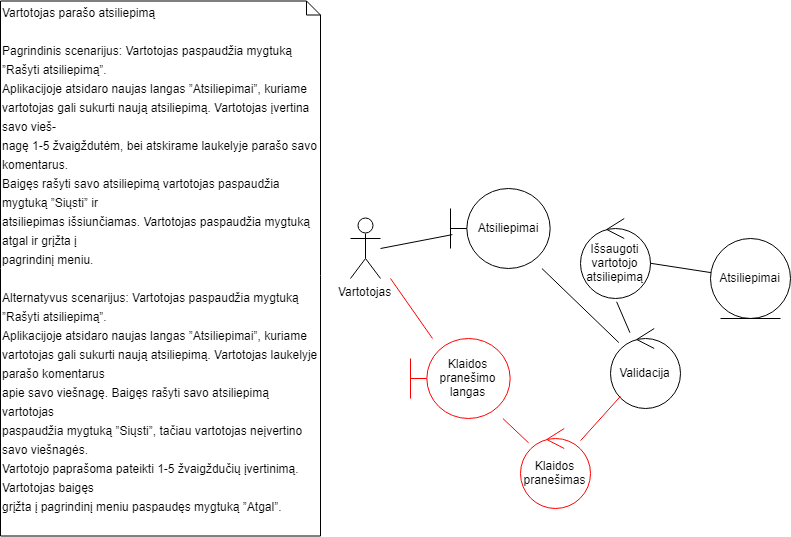
\includegraphics[width=1.0\textwidth]{rob12.png}
    \caption{UC: Vartotojas rašo atsiliepimą}
    \label{fig:rob12}
\end{figure}
\vskip 1cm

\begin{figure}[h]
    \centering
    \includegraphics[width=1.0\textwidth]{Robostiškumo14.png}
    \caption{UC: Vartotojas žiūri žemėlapį}
    \label{fig:rob14}
\end{figure}
\vskip 1cm

\begin{figure}[h]
    \centering
    \includegraphics[width=1.0\textwidth]{Robostiškumo15.png}
    \caption{UC: Vartotojas žiūri savo profilį}
    \label{fig:rob15}
\end{figure}
\vskip 1cm



\section{Eskizinio projekto peržiūra}
\subsection{Pataisytos robustiškumo diagramos}
\subsection{Pataisyta Domain diagrama}
\begin{figure}[h]
    \centering
    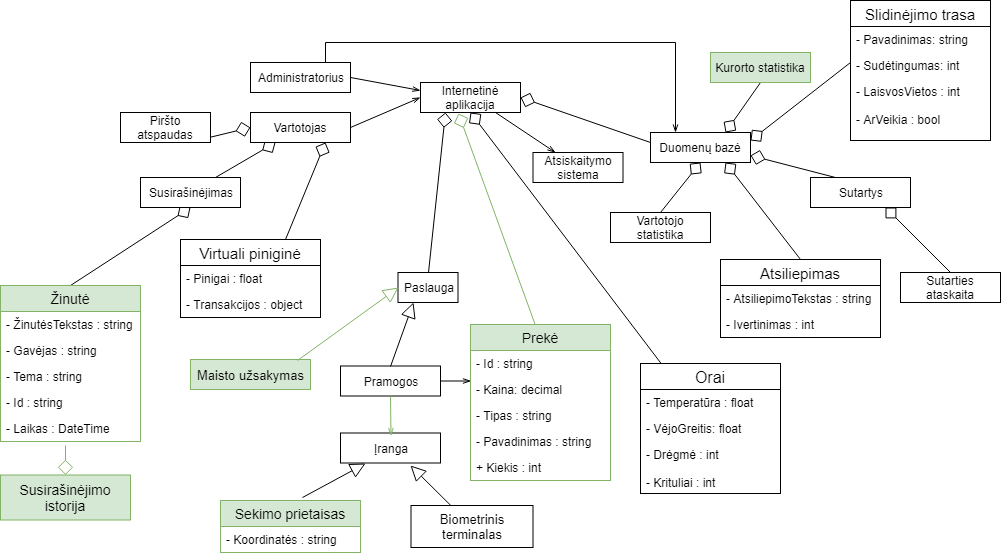
\includegraphics[width=1.0\textwidth]{domainfixed.png}
    \caption{Pataisyta Domain diagrama}
    \label{fig:domainfixed}
\end{figure}
\vskip 1cm


\section{Techninė architektūra}
\subsection{sistemos architektūra}
Sistema išskaidyta į 3 sluoksnius, View, controller ir model. View sluoksnyje talpiname vartotojo ir administratoriaus grafinius interfeisus, kurie bendrauja su Controller esančiais komponentais. Controller sluoksnyje esantys komponentai yra tarpiniai tarp grafinio interfeiso ir back-end, komponentai esantys jame gavę grafinio interfeiso signalus juos apdoroja ir kreipiasi į Model, kuriame esantys komponentai pagrinde skirti duomeų bazės redagavimui. Norint atvaizduoti atnaujintą informaciją vartotojui, model esantys komponentai perduoda informaciją į controller ir pastarasis perduoda informaciją view, kur ją išvysta vartotojas. 
\subsection{Išdestymo diagrama}
	\begin{figure}[h]
    \centering
    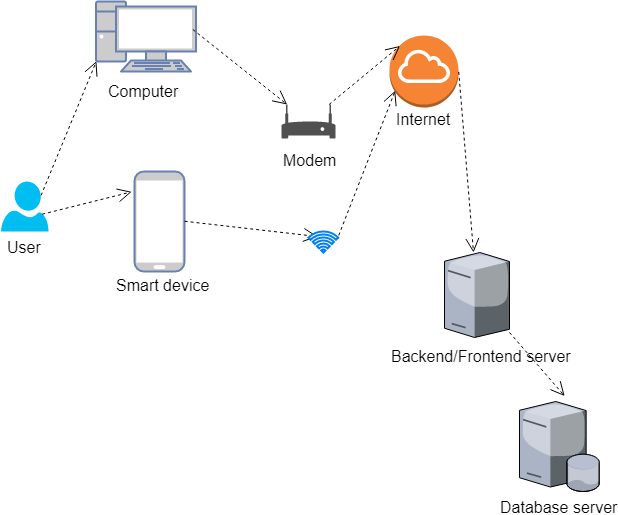
\includegraphics[width=1.0\textwidth]{Deployment.png}
    \caption{Pataisyta Domain diagrama}
    \label{fig:domainfixed}
\end{figure}
\subsection{Architektūriniai sprendimai}
\subsubsection{Front-end} Front-end'o kūrimui pasirinkome Javascript biblioteką ReactJS. Šią biblioteką pasirinkome dėl jos modularaus dizaino. Su React savo interfeisa galėsime išskaidyti į komponentus kas komandai leis lengviau įgyvendinti jį. Beto už šios bibliotekos vystyma yra atsakingi Facebook ir Instagram kas suteiks mums patikimumo norint ateityje keisti interfeisą. Ši biblioteka yra open source kas leis mums nemokamai naudoti juos.
\subsubsection{Back-end} Back-end'us rasyti naudosime ASP.NET Web API framework'a. Nes su šiuo framework'u dėl kelių priežasčių. Pirma - komanda jau naudojo šią technologija kituose projektuose ir yra susipažinusi kaip framework'as veikia. Antra - šis framework'as yra pakankamai lengvai naudojamas, paprasta kurti tiek mažas tiek didelias sisterma, todėl tai užtikrins plėtimasi ateityje. Trečia - kaina, šiuo metu ASP.Net framework'a programuotojams yra suteikiamas nemokamai. Nors šis framework'as ir nėra open source tačiau projektui nėra numatyta jokių išskirtinių elementų.


\end{document}